% PHY 3902 Experiment 3 Lab Report
% Author: Michelle Johnstone, Patrick Geraghty
% Affiliation: University of Ottawa
% Date: November 2, 2025

\documentclass[12pt,a4paper]{article}
\usepackage[utf8]{inputenc}
\usepackage{geometry}
\geometry{margin=1in}
\usepackage{graphicx}
\usepackage{amsmath}
\usepackage{hyperref}
\usepackage{listings}
\usepackage{xcolor}
\usepackage{float}
\usepackage[font=small,labelfont=bf,it]{caption}

% Python and Arduino code formatting
\lstset{
  basicstyle=\ttfamily\footnotesize,
  breaklines=true,
  frame=single,
  backgroundcolor=\color{gray!10},
  keywordstyle=\color{blue},
  commentstyle=\color{green!50!black},
  stringstyle=\color{red},
  numbers=left,
  numberstyle=\tiny\color{gray},
  captionpos=b,
  inputencoding=utf8
}

\begin{document}

% Title
\begin{center}
    {\LARGE\bfseries PHY 3902 Experiment 4 Lab Report}\\[1.5em]
    {\large Author(s): Michelle Johnstone, Patrick Geraghty}\\
    {\large Affiliation: University of Ottawa}\\
    {\large Date: November 2, 2025}
\end{center}

\section{Abstract}\label{sec:abstract}
This study evaluates the performance of a proportional-integral-derivative
(PID) control system for precise temperature regulation in an open system
using a cost-effective experimental setup.
The system comprises a thermistor for temperature sensing, a heating element,
and an Arduino microcontroller to implement the PID algorithm.
The PID approach dynamically adjusts the power supplied to the heating element
by accounting for proportional (\(k_p\)), integral (\(k_i\)), and derivative
(\(k_d\)) terms, enabling rapid and stable responses to temperature
fluctuations caused by environmental changes.
Experimental results demonstrated that the PID-controlled system maintained a
stable temperature with a standard deviation of \( \sigma = x \) and a percent
error of XX\%, significantly outperforming traditional on-off control methods.
Furthermore, the data were used to calculate the specific heat capacities of
aluminum (\(\frac{J}{g^{\circ}C}\)) and brass (\(\frac{J}{g^{\circ}C}\)),
showcasing the system's utility in thermodynamic measurements.
These findings underscore the potential of PID temperature control for
applications requiring high precision, adaptability, and energy efficiency in
dynamic environments.

\section{Introduction}\label{sec:introduction}
The standard on-off model of temperature control needs to be relatively
inaccurate with a large hysteresis otherwise the life span of circuitry
decreases proportionally with the temperature range.
The ability of the standard on-off model to maintain a set temperature is
severely diminished because of this, and they tend to work better for
realistic thermally isolated systems which don't need a large amount of power
to maintain the set temperature.
However, in this experiment the system is open to its environment and sudden
changes in temperature from external interaction, this is the benefit of PID
control, the system is able to react to these changes and adjust accordingly.
The first step is to make sure the power provided to the heater is
proportional to the amount needed for the set temperature, this helps to
prevent the heater from overshooting the temperature as the power supplied to
the heater decreases as it approaches the set temperature and increases as it
drops below the desired range.
The percentage of power applied is calculated using the error \(E\) as the
difference between the desired and measured temperatures over the width of the
allowed temperature band,

\begin{equation}
    E = \frac{T_{\text{set}} - T_{\text{measured}}}{\text{band}}\label{eq:error}
\end{equation}

which was used to control the amount of power supplied to the heater as a
percentage of the maximum amount of power.

\begin{equation}
    \text{Power} = ( T_{\text{offset}} + k_p E ) P_{\max}\label{eq:power_proportional}
\end{equation}

The factor \(k_p\) was added to control the effects of the error calculation
and control the speed with which the system reacts.
While this modification continues to produce a notable degree of error, it can
be observed that the temperature-time graph follows a decaying sinusoidal
function permits further refinement by integrating over an interval that is
twice the time required for the temperature to increase by an amount
equivalent to the band amplitude.
The integral of the error over this time interval

\begin{equation}
    I = \int {E } dt\label{eq:integral}
\end{equation}

can be used in conjunction with a proportionality constant \(k_i\) to avoid
overcorrecting the power and introducing new unwanted temperature
oscillations.
Adding this factor to equation~\eqref{eq:power_proportional} gives the
following formula for a more steady code for maintaining the set temperature.

\begin{equation}
    \text{Power} = (T_{\text{offset}} + k_p E + k_i I) P_{\max}\label{eq:power_integral}
\end{equation}

The final adjustment is to control the temperature when reacting to external
stimuli using derivative control.
If the temperature of the environment or the block suddenly spikes or drops,
this factor will allow the heater to react proportionally to the rate of
change of the error calculated by equation~\eqref{eq:error}.
This derivative \(D\) can be found by dividing the negative of the change in
error by the time interval over which this change is measured, the action time
of the code, using the following equation.

\begin{equation}
    D = - \frac{dE}{dx} = - \frac{\Delta{E}}{\Delta{x}}\label{eq:derivative}
\end{equation}

This value can be used in conjunction with an associated proportionality
constant \(k_d\) and introduced to equation~\eqref{eq:power_integral} to produce the final
equation for maintaining the set temperature

\begin{equation}
    \text{Power} = ( T_{\text{offset}} + k_p E + k_i I + k_d D) P_{\max}\label{eq:power_PID}
\end{equation}

In this experimental setup it is possible that the derivative control can
cause any noise in the temperature sensor to be amplified so it may be
beneficial to use a low value for the proportionality constant \(k_d\).

\section{Methods}\label{sec:methods}
\subsection{Experimental Setup}
\label{subsec:experimental-setup}

The experimental apparatus consisted of a heating element controlled via a
MOSFET, a thermistor for temperature measurement, and a microcontroller
running custom firmware to implement temperature control algorithms.
A wiring diagram of the complete setup is provided in
Figure~\ref{fig:setup_diagram}.

\begin{figure}[H]
    \centering
    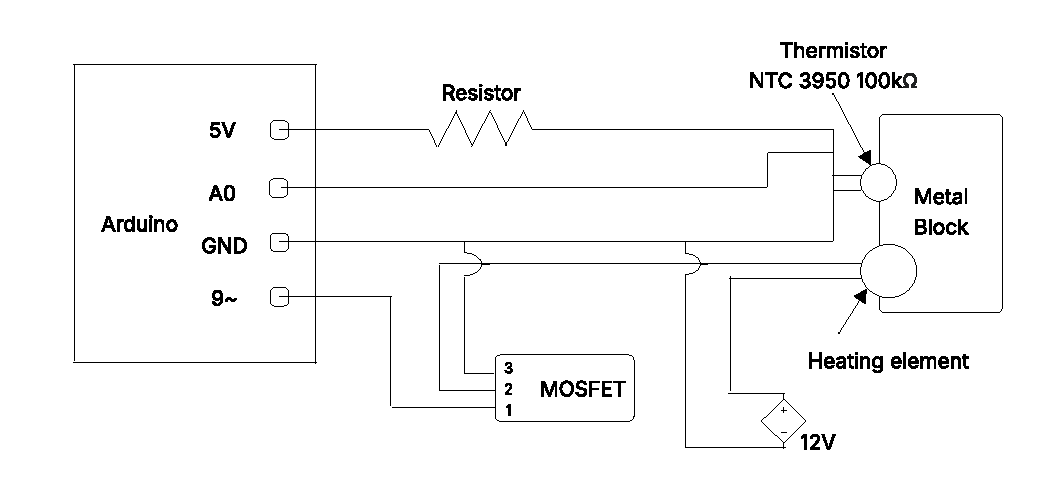
\includegraphics[width=0.8\textwidth]{PID_circuit_diagram}
    \caption{Wiring diagram of the experimental setup used for PID temperature control.}
    \label{fig:setup_diagram}
\end{figure}

\subsection{On-Off Control Baseline}
\label{subsec:on-off-control-baseline}

To establish a baseline response characteristic of the system, an on-off
control algorithm was implemented.
The heating element operated at maximum power until the thermistor registered
the set temperature of 65°C, at which point the heater was disabled until the
temperature dropped to the low temperature limit.
Temperature readings from the thermistor were recorded at approximately
one-second intervals and plotted as a function of time.
The expected behavior was characterized by a positive linear increase to a
peak above the set temperature, followed by a steeper decline back to the
lower temperature threshold, confirming proper circuit functionality.

\subsection{Proportional Control Implementation}
\label{subsec:proportional-control-implementation}

Following the baseline characterization, proportional control was implemented
using equation~\eqref{eq:power_proportional} to modulate heating power based
on the error between actual and set temperatures.
This approach reduced temperature oscillations by preventing full on-off
cycling and better maintained the temperature within the desired hysteresis band.
The proportionality constant \(k_p\) was initialized to 0.1 and incrementally
increased until measurable performance improvements were observed.
Despite these improvements, the system still exhibited a significant error
relative to the set temperature and continued to overshoot during each
oscillation cycle.

\subsection{System Response Time Characterization}
\label{subsec:system-response-time-characterization}

To optimize the integral control parameters, the system's reaction time was
determined using a step response method.
The reaction time was defined as the time required for the temperature to
reach 63\% of the total step change from baseline to target
temperature~\cite{step_response_wiki}.
A step input was applied by enabling the heating element to full power via the
MOSFET while continuously recording temperature measurements.
The initial temperature was measured using the thermistor, and the target
temperature was set to 5°C above this baseline value.
The time to reach the 63\% threshold was recorded as the system's response
time.
In accordance with laboratory guidelines~\cite{lab_guidelines}, the integral
action time constant was set to twice the measured response time to ensure
adequate system stabilization.

\subsection{Integral Control Refinement}
\label{subsec:integral-control-refinement}

Integral control was implemented to minimize the error and reduce the
oscillatory behavior observed with proportional control alone.
The integral constant \(k_i\) was initially set to approximately 0.0001 to
minimize the speed and magnitude of integral corrections, thereby reducing the
risk of integral windup~\cite{pid_integral_windup_controlcom} - a phenomenon
in which excessive error accumulation during actuator saturation leads to
overshooting and instability.
The integral constant was then gradually increased until the desired system
performance was achieved without overcorrection or instability.

\subsection{Derivative Control Optimization}
\label{subsec:derivative-control-optimization}

Derivative control was implemented to improve transient response and combat
sudden environmental temperature changes.
However, derivative action amplifies high-frequency noise in thermistor
measurements and measurement errors, potentially inducing unwanted
oscillations.
Therefore, the derivative constant \(k_d\) was initialized to 0.01 and
systematically decreased until the system ceased overreacting to measurement
noise while maintaining its ability to handle step changes in environmental
conditions.
Although derivative control is particularly beneficial for systems with
rapidly changing dynamics, its implementation in this relatively stable
thermal system required careful tuning to avoid amplifying measurement artifacts.

\subsection{Thermal Characterization}
\label{subsec:thermal-characterization}

Temperature-time response graphs were acquired at two different set
temperatures.
The voltage required to maintain each temperature was determined from the duty
cycle of the MOSFET at the stabilized portion of each response curve using
equation~\ref{eq:power_mosfet} to calculate the heat loss from the block.
Subsequently, the heating element was operated at full power using
Listing~\ref{lst:specific_heat_measurement} until a predetermined maximum
temperature was reached.
The time and power required to raise the temperature by 1°C were extracted
from these measurements.
These values were then substituted into equation~\ref{eq:specific_heat} to
determine the specific heat capacity of the test block.
Measurements at the two different temperatures allowed assessment of
temperature-dependent variations in specific heat capacity and estimation of
measurement uncertainty.

\section{Results and Discussion}\label{sec:results_and_discussion}
\subsection{On-Off Control Performance}
\label{subsec:on-off-control-performance}

The circuit was initially tested using a basic on-off control strategy to
maintain a target temperature of \(55^\circ\)C. As shown in
Figure~\ref{fig:baseline}, the system's temperature increased steadily over
time and eventually leveled off near the target temperature.

\begin{figure}[H]
    \centering
    \includegraphics[width=0.8\textwidth]{../out/baseline}
    \caption{
        Temperature vs. time for the on-off control circuit regulating an
        aluminum block to a target of $55^\circ$C. The system shows an
        oscillating temperature curve, with local minima just below the set
        temperature, demonstrating the basic performance of simple on-off
        control.
    }
    \label{fig:baseline}
\end{figure}

When hysteresis control was introduced, with a 3°C range around the target
temperature, the system exhibited a pattern of temperature fluctuations, as
shown in Figure~\ref{fig:hysteresis}.

\begin{figure}[H]
    \centering
    \includegraphics[width=0.8\textwidth]{../out/simple_hysteresis}
    \caption{
        Temperature vs. time for the on-off circuit with a 3$^\circ$C
        hysteresis band and a $55^\circ$C target. The plot shows
        characteristic oscillations as the heater cycles on and off,
        with sharp increases during heating phases and less pronounced drops
        during cooling.
    }
    \label{fig:hysteresis}
\end{figure}

The temperature increased steadily during heating but exceeded the upper limit
of the range before cooling down rapidly.
The temperature then dropped below the lower limit of the range before the
heater turned back on.
This uneven heating and cooling pattern suggests that the aluminum block loses
heat slower than it absorbs heat from the heater.
These results highlight the limited accuracy of simple on-off control methods
for maintaining a stable temperature in systems like this.
These measurements provided a baseline for comparing the performance of more
advanced control methods.

\subsection{Proportional Control Implementation}
\label{subsec:proportional-control-implementation2}

Proportional control was implemented to improve temperature regulation.
This method adjusts the heater's power based on how far the current
temperature is from the target.
Figure~\ref{fig:proportional_3_0.1} shows the system's behavior with a
proportionality factor (\(K_p\)) of 0.3, an offset of 0.1, and a temperature
range of 3°C. This approach reduced the size of temperature overshoots and
made the system more stable, although the offset value was not ideal for
keeping the temperature close to the target.

\begin{figure}[H]
    \centering
    \includegraphics[width=0.8\textwidth]{../out/proportional_0.1_offset}
    \caption{
        Temperature vs. time for proportional control with a 3$^\circ$C band,
        offset of 0.1, and $K_p = 0.3$ for an aluminum block at $55^\circ$C.
        The system exhibits reduced overshoot and improved stability compared
        to on-off control, but the offset is not fully optimized.
    }
    \label{fig:proportional_3_0.1}
\end{figure}

A further adjustment to the offset, increasing it to 0.165, improved the
performance, as shown in Figure~\ref{fig:proportional_3_0.165}.

\begin{figure}[H]
    \centering
    \includegraphics[width=0.8\textwidth]{../out/proportional_0.165_offset}
    \caption{
        Temperature vs. time for proportional control with a 3$^\circ$C band,
        offset of 0.165, and $K_p = 0.3$ for an aluminum block at $55^\circ$C.
        Improved offset tuning results in better temperature regulation and
        smaller fluctuations.
    }
    \label{fig:proportional_3_0.165}
\end{figure}

The system was able to stay within the target range for longer periods, and
the temperature fluctuations became smaller over time.
This behavior is typical of systems using proportional control, where the
heater's power is adjusted based on the difference between the current
temperature and the target, allowing for smoother changes compared to simple
on-off control.

The temperature range was then reduced to 1°C while keeping the same optimized
settings (\(K_p = 0.3\), offset = 0.165).
This adjustment allowed the system to regulate the temperature more precisely,
as shown in Figure~\ref{fig:proportional_1_0.165}.

\begin{figure}[H]
    \centering
    \includegraphics[width=0.8\textwidth]{../out/proportional_0.165_offset_1_band}
    \caption{
        Temperature vs. time for proportional control with a 1$^\circ$C band,
        offset of 0.165, and $K_p = 0.3$ for an aluminum block at $55^\circ$C.
        Narrowing the control band allows for more precise temperature
        regulation, though a small error remains.
    }
    \label{fig:proportional_1_0.165}
\end{figure}

However, the system still exhibited a small but consistent error, where the
temperature was slightly higher or lower than the target.
This occurred because proportional control requires a small difference between
the actual and target temperatures to maintain the heater's power and balance
heat loss to the environment.

\subsection{Proportional-Integral Control}
\label{subsec:proportional-integral-control}

To address the consistent temperature error observed with proportional
control, an integral control component was added.
Figures~\ref{fig:integral_1_0.165},
and~\ref{fig:live_plot_20251027_153510_integral}, show the performance of the
proportional-integral (PI) controller with \(K_p = 0.3\), \(K_i = 0.00001\),
an offset of 0.165, and a 1°C range, applied to the aluminum block at a target
temperature of \(55^\circ\)C. The integral control component works by
gradually correcting any long-term differences between the current temperature
and the target.

\begin{figure}[H]
    \centering
    \includegraphics[width=0.8\textwidth]{../out/integral_0.165_offset_1_band}
    \caption{
        Temperature vs. time for PI control with a 1$^\circ$C band, offset of
        0.165, $K_p = 0.3$, and $K_i = 0.00001$ for an aluminum block at
        $55^\circ$C. The addition of integral action reduces steady-state
        error and improves long-term stability.
    }
    \label{fig:integral_1_0.165}
\end{figure}

\begin{figure}[H]
    \centering
    \includegraphics[width=0.8\textwidth]{../out/live_plot_20251027_153510_integral}
    \caption{
        Temperature vs. time for PI control (Aluminum):
        $T_\text{set}=55^\circ$C, band=1, $K_p=0.3$, $K_i=0.00001$,
        offset=0.165. The plot demonstrates the system's ability to maintain
        temperature near the setpoint over time.
    }
    \label{fig:live_plot_20251027_153510_integral}
\end{figure}

This adjustment allowed the system to reduce the consistent error and
stabilize the temperature closer to the desired value.
Over time, the size of the temperature fluctuations decreased until the system
maintained a more stable performance near the target.

At a higher target temperature of \(65^\circ\)C, the PI controller with an
increased integral gain (\(K_i = 0.001\)) and an offset of 0.25 showed
effective performance, as illustrated in
Figure~\ref{fig:live_plot_20251029_163401}.

\begin{figure}[H]
    \centering
    \includegraphics[width=0.8\textwidth]{../out/live_plot_20251029_163401}
    \caption{
        Temperature vs. time for PI control at a higher setpoint ($65^\circ$C)
        with $K_p=0.3$, $K_i=0.001$, $K_d=0.0$, and offset=0.25. The increased
        integral gain enables faster correction of errors, demonstrating
        adaptability to different target temperatures.
    }
    \label{fig:live_plot_20251029_163401}
\end{figure}

The higher integral gain allowed faster correction of temperature errors,
demonstrating that the system could adapt effectively to different target
temperatures.

\subsection{Full PID Control and Derivative Action}
\label{subsec:full-pid-control-and-derivative-action}

The final step in the control strategy involved adding a derivative control
component, completing the proportional-integral-derivative (PID) system.
Derivative control helps the system respond more quickly to sudden changes in
temperature by predicting how the temperature is likely to change.
Figure~\ref{fig:live_plot_20251027_171632_derivative} shows the system's
behavior with the derivative gain set to zero (\(K_d = 0.0\)), effectively
functioning as a PI controller for comparison.

\begin{figure}[H]
    \centering
    \includegraphics[width=0.8\textwidth]{../out/live_plot_20251027_171632_derivative}
    \caption{
        Temperature vs. time for PID control (Aluminum):
        $T_\text{set}=55^\circ$C, band=1, $K_p=0.3$, $K_i=0.00001$, $K_d=0.0$,
        offset=0.165. With $K_d=0$, the system acts as a PI controller,
        providing a baseline for comparison with full PID control.
    }
    \label{fig:live_plot_20251027_171632_derivative}
\end{figure}

When derivative control was activated (\(K_d = 0.00001\)), the system
demonstrated a much faster response to sudden temperature changes, as shown in
Figure~\ref{fig:live_plot_20251028_162354}.

\begin{figure}[H]
    \centering
    \includegraphics[width=0.8\textwidth]{../out/live_plot_20251028_162354}
    \caption{
        Temperature vs. time for PID control (Aluminum):
        $T_\text{set}=55^\circ$C, band=1, $K_p=0.3$, $K_i=0.00001$,
        $K_d=0.00001$, offset=0.165. Activating derivative control results in
        a faster response to sudden temperature changes, maintaining a much
        tighter oscilation around the setpoint.
    }
    \label{fig:live_plot_20251028_162354}
\end{figure}

For instance, during testing, the temperature sensor was removed from the
aluminum, causing it to detect a rapid drop in temperature.
The derivative control responded by immediately increasing the heater power to
100\%, highlighting its ability to handle unexpected changes.
This response occurred with \(K_d = 0.001\), showing that even small
derivative gains have a significant effect on how the system reacts to sudden
events.

However, the derivative control also introduced a drawback: it amplified
small fluctuations in the temperature readings caused by sensor noise.
This resulted in slightly more variability in the heater's power during normal
operation, which partially reduced the benefits of the faster response to
temperature changes.

The PID controller was also tested on a brass block at \(65^\circ\)C, using
\(K_p = 0.3\), \(K_i = 0.001\), \(K_d = 0.001\), and an offset of 0.25, as
shown in Figure~\ref{fig:live_plot_20251029_170448}.

\begin{figure}[H]
    \centering
    \includegraphics[width=0.8\textwidth]{../out/live_plot_20251029_170448}
    \caption{
        Temperature vs. time for PID control (Brass):
        $T_\text{set}=65^\circ$C, band=1, $K_p=0.3$, $K_i=0.001$, $K_d=0.001$,
        offset=0.25. The PID controller successfully regulates the temperature
        of a brass block, demonstrating adaptability to different materials.
    }
    \label{fig:live_plot_20251029_170448}
\end{figure}

The PID controller successfully regulated the temperature of the brass block,
demonstrating its ability to adapt to materials with different thermal properties.

\subsection{Specific Heat Capacity Measurements}
\label{subsec:specific-heat-capacity-measurements}

The specific heat capacity determinations yielded results with substantial
deviations from accepted literature values.
For the aluminum block (\(24.64 \pm 0.005\) g), the calculated specific heat
capacity was \(1.8 \, \frac{\text{J}}{\text{g}\cdot{}^\circ\text{C}}\),
representing a 100\% error relative to the accepted value of
\(0.9 \, \frac{\text{J}}{\text{g}\cdot{}^\circ\text{C}}\)~\cite{specific_heat}.
Similarly, the brass block (\(72.35 \pm 0.005\) g) yielded
\(0.8 \, \frac{\text{J}}{\text{g}\cdot{}^\circ\text{C}}\) compared to the
literature value of \(0.4 \, \frac{\text{J}}{\text{g}\cdot{}^\circ\text{C}}\)
~\cite{specific_heat}, again corresponding to a 100\% error.

While it was noted that aluminum measurements typically exceed
theoretical values in this experimental setup, the magnitude of the
discrepancies suggests systematic error rather than random uncertainty.
Potential error sources include: (1) inaccuracies in PWM-to-power conversion
calculations, (2) errors in MOSFET switching efficiency modeling, (3)
miscalibration of the energy delivery measurement, (4) unaccounted heat losses
to the environment during the heating interval, or (5) noise amplification in
the data acquisition chain affecting temperature change rate calculations.

Experimental limitations prevented comprehensive error analysis through
extended data collection.
Hardware failures during the experiment, including damaged components
requiring replacement, significantly compressed the available testing time.
A more extensive measurement campaign spanning a wider temperature range would
have facilitated identification of whether errors exhibited systematic trends
or random scatter, thereby isolating the dominant uncertainty source.
The consistent overestimation for both materials suggests a systematic
calibration error in the power delivery measurement or energy calculation
algorithm rather than material-specific measurement artifacts.


\section{Conclusion}\label{sec:conclusion}
In conclusion, the Arduino-based PID temperature control system effectively
demonstrated progressive improvements in stability and response across the
ON--OFF, P, PI, and PID configurations.
The PI controller achieved the most stable performance, maintaining the target
temperature with the smallest standard deviation and least noise reactivity,
validating its theoretical advantages.
However, the experimentally determined specific heat capacities for aluminum
and brass were significantly higher than accepted values, primarily due to
systematic errors.
These could have included code-related issues such as the chosen constants or
improper power scaling of the PWM signals, circuitry losses through the MOSFET
and wiring, limited thermal insulation, and sensor inaccuracies from the
thermistor.
Had there been more time for the experiment it could have proven beneficial to
incorporate direct voltage and current measurements for accurate power
determination, improved sensor calibration, and refined control code to
eliminate offset bias.
Despite these discrepancies, the experiment successfully demonstrated the
principles and effectiveness of PID-based temperature regulation.

% Bibliography
\bibliographystyle{plain}
\bibliography{../docs/references}

% Supplementary Code
\appendix
\section{Supplementary Code}\label{sec:supplementary-code}
\subsection*{Python Scripts}

\lstinputlisting[language=Python,caption={temp\_plot.py: Python script to analyze and plot temperature data.},label={lst:temp_plot}]{../src/temp_plot.py}
\lstinputlisting[language=Python,caption={specific\_heat\_capacity.py: Python script to calculate specific heat capacity from temperature data.},label={lst:specific_heat_capacity}]{../src/specific_heat_capacity.py}

\subsection*{Util Classes}

\lstinputlisting[language=Python,caption={constants.py: Shared constants},label={lst:constants}]{../src/utils/constants.py}
\lstinputlisting[language=Python,caption={data\_processor.py: Util functions for interpretting temperature data.},label={lst:data_processor}]{../src/utils/data_processor.py}
\lstinputlisting[language=Python,caption={specific\_heat\_calc.py: Util functions for calculting specific heat capacities from temperature data.},label={lst:specific_heat_calc}]{../src/utils/specific_heat_calc.py}

\subsection*{Arduino Sketches}

\lstinputlisting[language=C++,caption={CSVPrinter.h: Custom header file to facilitate easy csv output to the serial monitor.},label={lst:CSVPrinter}]{../src/Temp_ON_OFF_integral/CSVPrinter.h}
\lstinputlisting[language=C++,caption={Temp\_ON\_OFF\_integral.ino: Full PID control for Arduino Uno.},label={lst:Temp\_ON\_OFF\_integral}]{../src/Temp_ON_OFF_integral/Temp_ON_OFF_integral.ino}
\lstinputlisting[language=C++,caption={response\_time\_measurement.ino: Simple Arduino sketch to determine the response time of a heating system.},label={lst:response_time_measurement}]{../src/response_time_measurement/response_time_measurement.ino}
\lstinputlisting[language=C++,caption={specific\_heat\_measurement.ino: Simple Arduino sketch to apply constant heating cycles to a heater.},label={lst:specific_heat_measurement}]{../src/specific_heat_measurement/specific_heat_measurement.ino}


% End of document
\end{document}
